\titledquestion{Diode Rectifier}

Our neural network needs a way to introduce a \emph{cutoff} so that it can make different ``decisions'' depending on the input. Without this, the entire network would reduce to one big weighted sum, which is far too simple to represent interesting functions. To add this cutoff, we will use a \textbf{diode rectifier}: a circuit that passes positive voltages through but forces all negative voltages to zero.

This is actually very close to a function used in real artificial neural networks (including large language models like ChatGPT), called a \textbf{ReLU} (Rectified Linear Unit):

\begin{center}
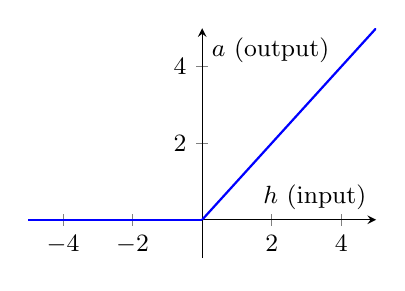
\begin{tikzpicture}
    \begin{axis}[
        width=6cm, height=4.5cm,
        xlabel={$h$ (input)}, ylabel={$a$ (output)},
        axis lines=center,
        xmin=-5, xmax=5, ymin=-1, ymax=5,
        xtick={-4,-2,0,2,4}, ytick={0,2,4},
        every axis plot/.append style={thick},
        font=\small,
    ]
    \addplot[blue, domain=-5:0] {0};
    \addplot[blue, domain=0:5] {x};
    \end{axis}
\end{tikzpicture}

$a = \max(0,\; h)$
\end{center}

Our diode version isn't perfect --- it has a $\sim$0.6V dead zone due to the diode's forward voltage drop --- but this isn't critical; the network can still represent any function.

Assemble the circuit in Figure \ref{fig:rectifier} on your breadboard. Use a 1N4148 signal diode and a 10\si{\kilo\ohm} pull-down resistor. \textbf{Build 2 of these} --- one per hidden neuron.

For testing, connect a 1kHz 5$V_{pp}$ sine wave from the signal generator to the input.

\begin{figure}[h]
    \centering
    \begin{circuitikz}[scale=1.3, transform shape, american]
        % Input
        \draw (-3, 0) to[sV, v_=$V_{in}$ (\texttt{W1})] ++(0,-2) node[sground] {};
        \draw (-3, 0) to[short, -o] ++(-0.5, 0) node[left] {In};
        \draw (-3, 0) to[diode, l=1N4148] ++(3, 0) coordinate (out_node);

        % Output
        \draw (out_node) to[short, -o] ++(1, 0) node[right] {Out ($a$)};

        % Pull-down resistor
        \draw (out_node) to[R, l_=10k$\Omega$, *-] ++(0, -2) node[sground] {};
    \end{circuitikz}
    \caption{Bare diode rectifier with pull-down resistor. When $V_{in} > 0.6$V, the diode conducts and the output follows the input (minus the diode drop). When $V_{in} < 0.6$V, the diode is reverse-biased and the pull-down resistor holds the output at 0V.}
    \label{fig:rectifier}
\end{figure}

Connect CH1 to the input and CH2 to the output.

In WaveForms, set the Wavegen to Sine with $f = 1$kHz and amplitude = 5V. For the scope, set your CH1 range to 1V/div.

\pagebreak
\begin{parts}
\part[3] Paste a screenshot of your oscilloscope showing the rectification of the sine wave. Both the input and output waveforms should be clearly visible.

\makessbox{5cm}
\medbreak

\part[2] Explain what the circuit does: what happens to positive input voltages? What happens to negative input voltages? How does the diode accomplish this?

\makeemptybox{3cm}
\end{parts}

\pagebreak
